\documentclass[11pt]{report}
% \usepackage[utf8]{inputenc} % pictures
\usepackage[titletoc]{appendix} % appendix
\usepackage{nopageno} % Disable bottom page #
\usepackage{multicol} % multicolumn 
\usepackage{enumitem} % list items
\usepackage{fancyhdr} % page headers
\usepackage{titlesec} % title format

% Graphics library for displaying pictures
\usepackage{graphicx}
\graphicspath{ {images/} }

\usepackage{tabu} % allows for tables with width control

% Setting the margins
\usepackage[top=.5in, left=1in, bottom=1in, right=1in]{geometry}
 
% bibliography stuff, to compile use
% user@host~$ pdflatex file.tex
% user@host~$ bibtex file.tex 
% user@host~$ pdflatex file.tex
%
\usepackage[backend=bibtex]{biblatex}
\addbibresource{final_report.bib}

% Create clickable table of contents
\usepackage{hyperref}
\hypersetup {colorlinks,
    citecolor=black,
    filecolor=black,
    linkcolor=black,
    urlcolor=black
}

% Fix itemize spacing
\newenvironment{myitemize}
{ \begin{itemize}
    \setlength{\itemsep}{0pt}
    \setlength{\parskip}{0pt}
    \setlength{\parsep}{0pt}     }
{ \end{itemize}                  } 

%set font style
\renewcommand\familydefault{\sfdefault}

% Set line spacing
\renewcommand{\baselinestretch}{1}

% Set indent size
\setlength\parindent{0pt}

% column spacing
\setlength\columnsep{4pt}

% Title format
\titleformat{\chapter}{\Huge\bf}{\thechapter}{20px}{\Huge\bf}


\begin{document}
% Begining of title page

{\Huge \textbf{CS 320 Course Project Final Report:}}
\vspace{5mm}
\begin{flushright}

    {\huge for}
    \vspace{20mm}

    \textbf{\Huge Vaultron}
    \vspace{20mm}

    {\huge Version $<0.0.1>$}
    \vspace{20mm}

    {\huge Prepared by}
    \vspace{20mm}

    \textbf{\huge Cryptomaniacs}
    \vspace{20mm}
\end{flushright}

\begin{multicols}{3}
    \noindent
    \begin{itemize}
        \item[] {\Large Colton King}
        \item[] {\Large Grant Wade}
        \item[] {\Large Robby Boney}
        \item[] {\Large Rob Wooner}
    \end{itemize}

    \begin{itemize}
        \item[] {\Large 11245746}
        \item[] {\Large 11435949}
        \item[] {\Large 11453444}
        \item[] {\Large 11496643}
    \end{itemize}

    \begin{itemize}
        \item[] {\Large\texttt colton.king@wsu.edu}
        \item[] {\Large\texttt grant.wade@wsu.edu}
        \item[] {\Large\texttt robby.boney@wsu.edu}
        \item[] {\Large\texttt robert.wooner@wsu.edu}
    \end{itemize}
\end{multicols}

\vfill

\begin{flushright}
    \vspace{20mm}
    {\Large \textbf{Date:} Sunday, December 10th, 2017}
\end{flushright}

% Begining of second page
\clearpage


\tableofcontents{}

\chapter{Introduction}

\section{Project Overview}
Vaultron is a cryptographically secure cross platform password manager
written in electron and node.js which allows users to store their account
information for websites locally with easy access. It will store hashed passwords 
in a JSON file for safe keeping. Vaultron will allow multiple profiles, each one will
have a master password of its own that will unlock The Vault. This master password will 
let the user not only let them access their passwords, but also edit any information that 
is stored in The Vault. The master password will be created by the user so that they can 
remember it. Our password manager also allows the user to create and store strong and 
secure passwords that are created with our password generator. This allows the user 
to only need to remember the master password. 



\section{Definitions, Acronyms And Abbreviations}
\textbf{CSS:} Cascading Style Sheets, used to style our electron application

\textbf{Electron:} Cross platform desktop application development environment
using HTML, CSS, and JavaScript

\textbf{node.js:} JavaScript runtime built on Chrome's V8 JavaScript engine. Used
for file io and backend applications.

\textbf{HTML:} HyperText Markup Language, used to design our electron application

\textbf{JavaScript:} Programming language used on the web and Electron

\textbf{Vault:} Password storage platform created for this project

\textbf{PBKDF2:} Password Based Key Derivation Function v2


\section{References And Acknowledgments}

    \nocite{*}
    \printbibliography[heading=none]



% END OF INTRODUCTION

\chapter{Design}

\section{System Modeling}
At the 



\section{Interface Design}
Following are visualizations the windows for our application and brief 
descriptions of their purpose to the app.

\subsection{Login}
This window is where the user starts from and allows them to create an account
or login into a previously existing one with their masterpassword.

\begin{center}
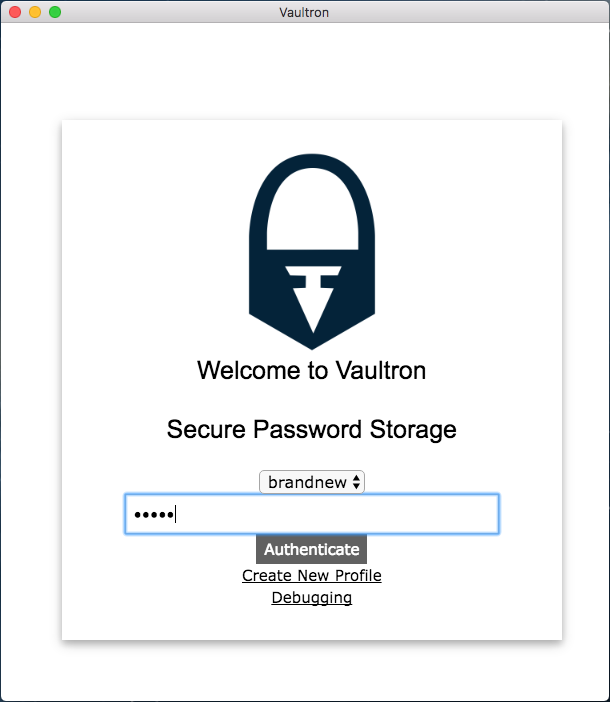
\includegraphics[scale=0.50]{app-login-demo.png}
\end{center}

\subsection{Main App}
The main window that displays the vault content and allows the user to navigate
to other aspects of the app such as password generation or entry creation.

\begin{center}
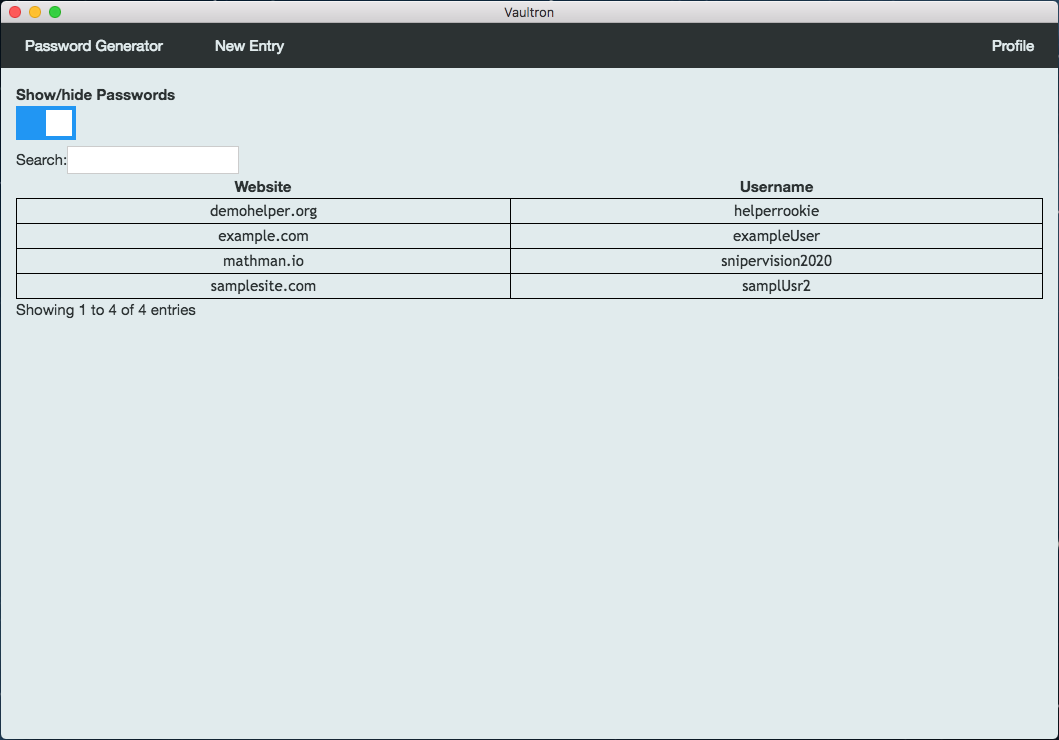
\includegraphics[scale=0.40]{app-main-demo.png}
\end{center}

\subsection{Create Entry}
This window is used to add information to be stored in the vault.
\begin{center}
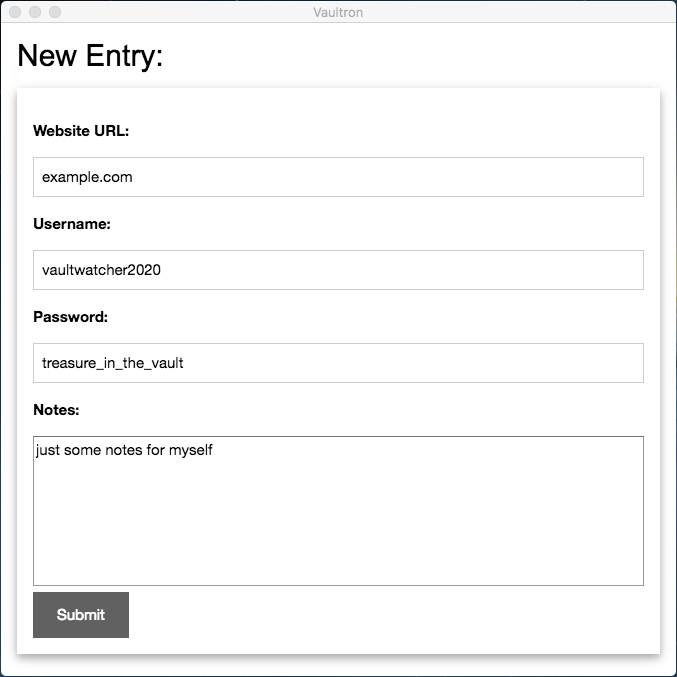
\includegraphics[scale=0.40]{app-newentry-demo.png}
\end{center}

\subsection{Generate Password}
Our tool for users to generate cryptographically secure passwords which can be
used in place of user designed passwords.
\begin{center}
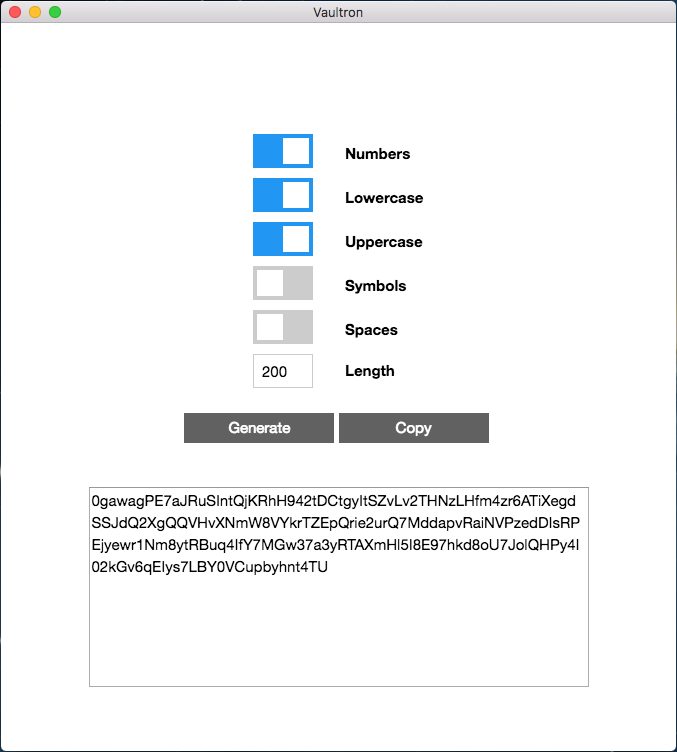
\includegraphics[scale=0.40]{app-passgen-demo.png}
\end{center}

% END OF DESIGN

\chapter{Implementation}
\section{Development Environment}

Our tools for this project involved:

\begin{itemize}
    \item \textbf{Electron} - Open Source javascript framework for cross platform app development
    \item \textbf{Node.js} - backend javascript runtime
    \item \textbf{CSS3 \& HTML5} - App styling and layout
    \item \textbf{Latex} - used to write the reports/documents and generate pdfs
    \item \textbf{IDS} - IDE's used by our team 
        \begin{itemize}
            \item Sublime Text
            \item VSCode
            \item Atom
        \end{itemize}
\end{itemize}


\section{Task Distribution}

\subsection{Colton King}
My primary contribution to this app was helping with the creating of the layout
and implemting buttons. I wrote the original new entry feature for this app 
that eventualy got updated and changed as we progressed. I also helped with 
the documentation for this app.
\subsection{Grant Wade}

\subsection{Robby Boney}
My primary contribution to this app was layout and css styling as well as the 
code and implementation of the password generation page. In addition to this
I contributed to the main table where the data is displayed.

\subsection{Rob Wooner}
My efforts in this project was focused around Vaultrons main page. I helped
Robby with the layout and configuration of the data table presented on the main
page. Along with the contributions listed above, I also took part in the creation 
and drafting of the documentation for Vaultron.



\section{Challenges}
Developing this application has been the first real experience for all of us
developing software in a larger group setting. This has introduced us to new
obstacles such as work delegation and differences in coding styles. These posed
useful for us to adapt to because most of our previous experience only relied
on our own ability to code a project, whereas this larger scale project 
required a much higher level of teamwork that brought us together as friends
and gave us expereince dealing with these software development challenges.


% END OF IMPLEMENTATION


\chapter{Testing}

\section{Testing Plan}
Our static testing process involved testing the consistency of the source code 
and HTML pages by testing syntax and usability of the code elements such as 
valid links and no unused variables. The dynamic testing process involved
testing user interface elements such as buttons and input fields as well as 
code functionality through a custom interactable encryption and decryption
testing suite.


\section{Tests For Functional Requirements}

\subsection{Generate Secure Passwords}
Password generation will allow the user to generate a secure password of any length or 
complexity. This will be accomplished using the secure bytes provided by every
operating system. There will be options to include special characters, uppercase,
lowercase, and numbers when generating the passwords.

\subsection{Authenticate User to Decrypt Passwords}
This function will verify who the user is before decrypting any passwords, utilizing 
the master password provided by the user. Once the master password is verified
the master key will be decrypted to make all passwords avaliable.

\subsection{Generate a Vault on First Run of Software}
This function will create a Vault every time a new user is registered for an account 
with Vaultron. This is a database created for the user to be able to create new
passwords, search, delete, copy (to the clipboard), and manipulate their passwords
for any account as they deem necessary.

\subsection{Search Through Passwords}
This function will allow the user to search through their already created passwords
with either the website the password is attached to or the username that goes with 
the password. 

\subsection{Creation of New Entries}
This function allows the user to create new entries to there previously created 
database. They will need to input the website that is using the password and
username that accompanies the password.  They can either store a password that
they provide or use the password generater and generate a new password.

\subsection{Syncing Users Vaults Between Computers}
This function allows the user to acquire their Vaultron account from any computer 
they want, utilizing which ever resource they are most comfortable using. (Dropbox, 
Google Drive, etc)

% END functional requirements


\section{Tests For Non-Functional Requirements}
All non-functional requirements passed our testing. Log-in time was declared to 
take less than 2 seconds, which our inspector verified by running the app. In 
addition to log-in, our inspector tested the time it took to make a entry which 
was less than 1 second. Lastly our inspector verified that generating a new 
password took less 1 second. Through these tests we were able to verify that our 
non-functional tests were passed.

\section{Hardware And Software Requirements}
Our app is cross platform and therefore does not have hardware requirements. 
Since the app is cross platform, our software requirements will involve 
testing on multiple operating systems including Windows 10 and MacOS Sierra.

% END OF TESTING


\chapter{Analysis}

\subsection*{UI Design}
\begin{itemize}
    \item Colton: 10 hours
    \item Grant: 12 hours
    \item Rob: 18 hours
    \item Robby: 24 hours
\end{itemize}

\subsection*{File Operations}
\begin{itemize}
    \item Colton: 10 hours
    \item Grant: 10 hours
    \item Rob:  6 hour
    \item Robby: 6 hours
\end{itemize}

\subsection*{Implementation of Security}
\begin{itemize}
    \item Colton: 10 hours
    \item Grant: 40 hours
    \item Rob: 10 hours
    \item Robby: 10 hours
\end{itemize}



% END OF Analysis


\chapter{Conclusion}
This project has been a eye opening experience for our team. The challenge of combining our skills together to make a cohesive product together showed us how difficult it can be to coordinate work within a group and design an application that everyone in the group approves in regards to functionality and layout. Beyond the task of internal organization we also learned how users who have not worked on coding our app, viewed it during the inclass presentations. This was a very important aspect this project because it gave us first hand experience interacting with people who do not see our project the same way we do and allowed us to adapt our application to include good ideas from others we had never thought us which ultimately made our app more secure and visually appealing.

% END OF CONCLUSION


\begin{appendices}

    \chapter{Group Log}
    \begin{itemize}
        \item Meeting 1: Sunday, October 8th: Discussed project ideas and began writing SRS. 3 hours
        \item Meeting 2: Monday, October 9th: Finished first two chapters of SRS. 1 hour
        \item Meeting 3: Wednesday, October 11th: Wrote majority of chapters 3 and 4. 2 hours
        \item Remote Work: 10-12 hours via Discord/Github
        \item Colton: Wrote sections 1.2, 2.6, 3.1.1, 3.1.2, 4.1, Data dictionary
        \item Grant: Designed SRS, and wrote sections 1.3, 2.7, 3.1.4, 4.2, 4.3
        \item Rob: Designed SRS, and wrote sections 2.3, 2.5, 3.1.3, 3.2, 3.3
        \item Robby: Designed diagrams, references, and wrote sections 1.5, 1.6, 2.1, 2.4, 3.3.1
    \end{itemize}


\end{appendices}

\end{document}
